\documentclass{standalone}
\usepackage{pgfplots}
\pgfplotsset{compat=newest}
\usepgfplotslibrary{patchplots}
\begin{document}
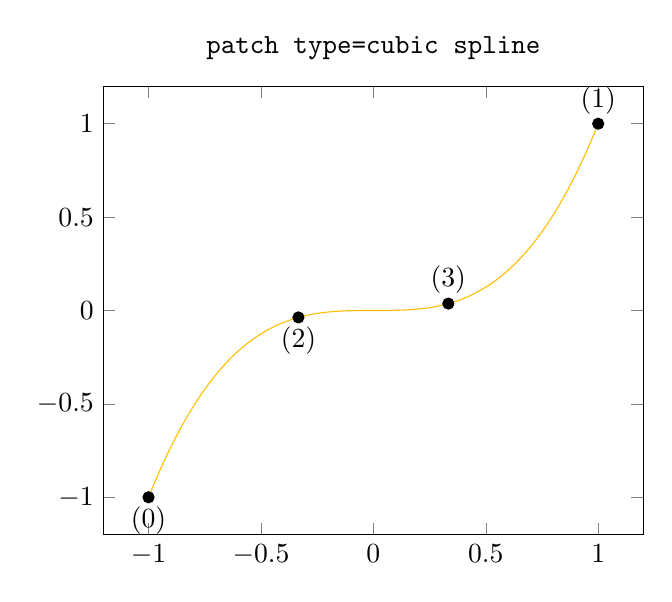
\begin{tikzpicture}
\begin{axis}[nodes near coords={(\coordindex)},
	title={\texttt{patch type=cubic spline}}]
\addplot[
	mark=*,
	patch,mesh,
	patch type=cubic spline]
coordinates {
	% left, right, left middle, right middle
	(-1,-1) 
	(1,1)  
	(-1/3,{(-1/3)^3})
	(1/3,{(1/3)^3})
};
\end{axis}
\end{tikzpicture}
\end{document}
